%% fig_pencil.tex -- the pencil of quaternionic loci inside D_{2,2}.  Left: a
%% stack of Siegel threefolds S_k, one for each k, drawn as plates inside the
%% four-dimensional family, with the two members carrying a rational point
%% marked.  Right: the invariant mu_k / beta(k) is constant along the pencil
%% while the degree bound grows linearly in k.
\documentclass[tikz,border=9pt]{standalone}
\usepackage{amsmath,amssymb}
\usetikzlibrary{arrows.meta,calc,backgrounds,positioning}
%% palette.tex -- shared colour definitions for the figures
\definecolor{PInk}{RGB}{26,32,44}
\definecolor{PBlue}{RGB}{37,82,139}
\definecolor{PTeal}{RGB}{23,127,125}
\definecolor{POchre}{RGB}{193,138,44}
\definecolor{PClay}{RGB}{178,74,58}
\definecolor{PSlate}{RGB}{108,122,137}
\definecolor{PViolet}{RGB}{110,86,150}
\definecolor{WBlue}{RGB}{223,234,246}
\definecolor{WTeal}{RGB}{220,238,236}
\definecolor{WOchre}{RGB}{250,240,218}
\definecolor{WClay}{RGB}{247,229,224}
\definecolor{WSlate}{RGB}{238,241,244}
\definecolor{PMag}{RGB}{158,58,110}
\definecolor{PGrass}{RGB}{62,124,66}
\definecolor{PAmber}{RGB}{214,112,38}
\definecolor{PIndigo}{RGB}{58,64,140}
\definecolor{PRule}{RGB}{176,186,197}

%% shared macros so the standalone figures match the paper
\providecommand{\QQ}{\mathbb{Q}}
\providecommand{\ZZ}{\mathbb{Z}}
\providecommand{\RR}{\mathbb{R}}
\providecommand{\CC}{\mathbb{C}}
\providecommand{\PP}{\mathbb{P}}
\providecommand{\Kx}{K^{\times}}
\providecommand{\HW}{W}
\providecommand{\Nm}{\mathrm{N}}
\providecommand{\Hdg}{\mathrm{Hdg}}
\providecommand{\NS}{\mathrm{NS}}
\providecommand{\cA}{\mathcal{A}}
\providecommand{\cD}{\mathcal{D}}
\providecommand{\cF}{\mathcal{F}}
\providecommand{\cP}{\mathcal{P}}
\providecommand{\cO}{\mathcal{O}}
\providecommand{\cQ}{\mathcal{Q}}
\providecommand{\bbar}[1]{\overline{#1}}
\providecommand{\ch}{\operatorname{ch}}
\providecommand{\End}{\mathrm{End}}


\tikzset{obl/.style={x={(1cm,0cm)}, y={(0.52cm,0.36cm)}, z={(0cm,1cm)}}}

%% a thin plate: corner (x0,y0,z0), width w, depth p, thickness t, style
\newcommand{\plate}[7]{%
  \begin{scope}[obl]
    \fill[#7 top]   (#1,#2,#3+#6) -- (#1+#4,#2,#3+#6) -- (#1+#4,#2+#5,#3+#6) -- (#1,#2+#5,#3+#6) -- cycle;
    \fill[#7 front] (#1,#2,#3) -- (#1+#4,#2,#3) -- (#1+#4,#2,#3+#6) -- (#1,#2,#3+#6) -- cycle;
    \fill[#7 side]  (#1+#4,#2,#3) -- (#1+#4,#2+#5,#3) -- (#1+#4,#2+#5,#3+#6) -- (#1+#4,#2,#3+#6) -- cycle;
    \draw[#7 edge]  (#1,#2,#3) -- (#1+#4,#2,#3) -- (#1+#4,#2,#3+#6) -- (#1,#2,#3+#6) -- cycle;
    \draw[#7 edge]  (#1+#4,#2,#3) -- (#1+#4,#2+#5,#3) -- (#1+#4,#2+#5,#3+#6) -- (#1+#4,#2,#3+#6);
    \draw[#7 edge]  (#1,#2,#3+#6) -- (#1,#2+#5,#3+#6) -- (#1+#4,#2+#5,#3+#6);
  \end{scope}}

\tikzset{
  fam top/.style={fill=WSlate!60}, fam front/.style={fill=WSlate!80!PSlate!20},
  fam side/.style={fill=WSlate!60!PSlate!30}, fam edge/.style={draw=PSlate,line width=0.5pt,dashed},
  sk top/.style={fill=WTeal},  sk front/.style={fill=WTeal!80!PTeal!35},
  sk side/.style={fill=WTeal!60!PTeal!45}, sk edge/.style={draw=PTeal,line width=0.6pt},
  rq top/.style={fill=WOchre}, rq front/.style={fill=WOchre!80!POchre!35},
  rq side/.style={fill=WOchre!60!POchre!45}, rq edge/.style={draw=POchre,line width=0.9pt},
}

\begin{document}
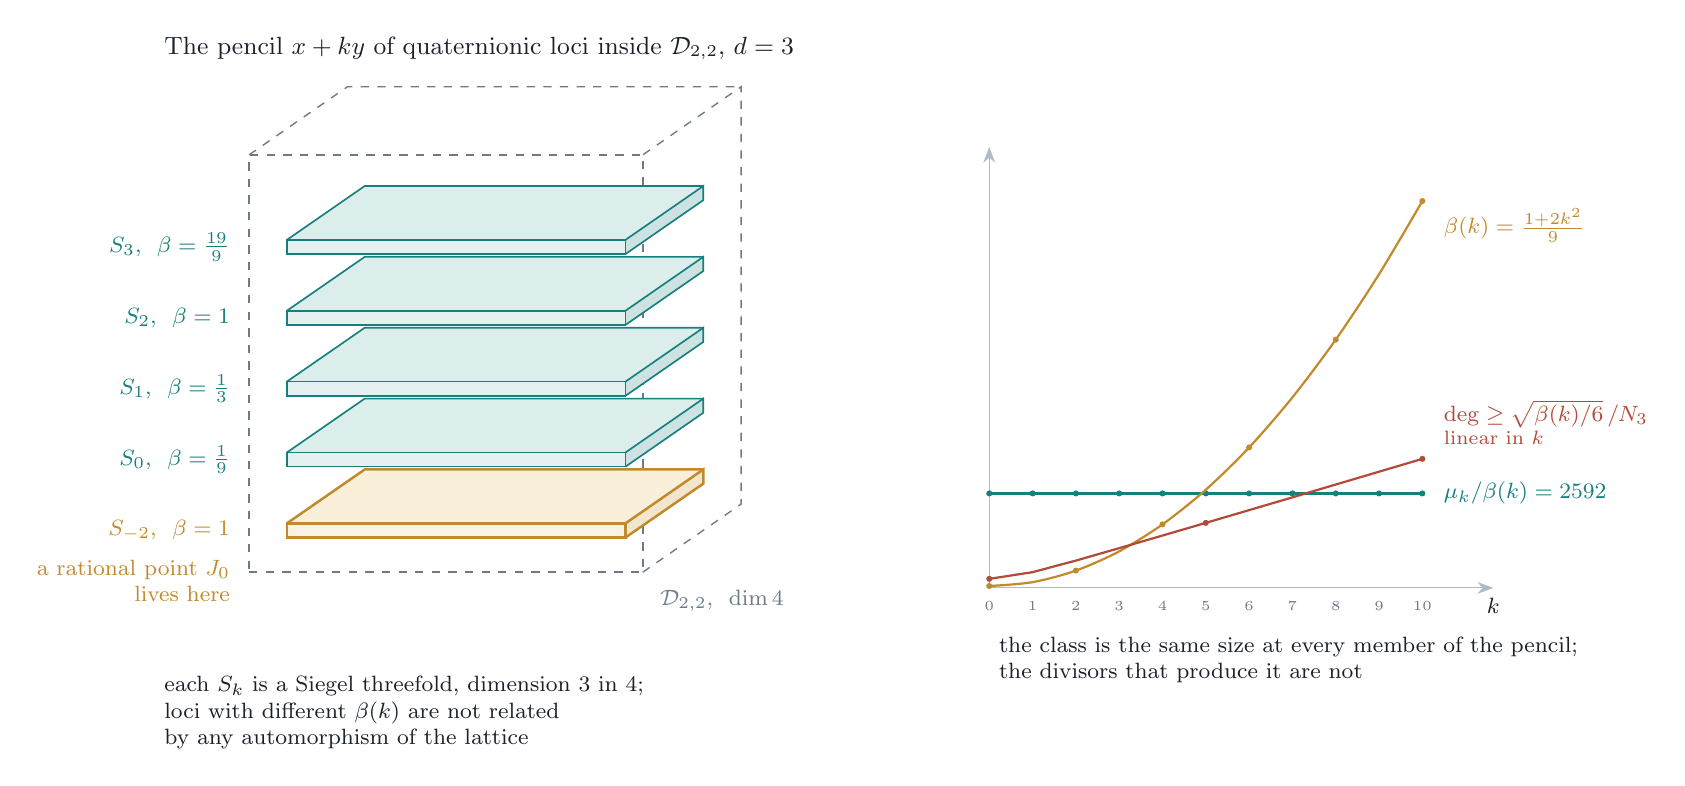
\begin{tikzpicture}[font=\small,text=PInk]

%% =====================================================================
%% Left: the family as a box, the pencil as plates inside it.
%% =====================================================================
\node[anchor=west,font=\small,text=PInk] at (-1.2,5.75)
  {The pencil $x+ky$ of quaternionic loci inside $\mathcal{D}_{2,2}$, $d=3$};

% the ambient family, drawn as a translucent box (dim 4, drawn as 3)
\begin{scope}[obl]
  \draw[PSlate,dashed,line width=0.5pt] (0,0,-0.9) -- (5,0,-0.9) -- (5,0,4.4) -- (0,0,4.4) -- cycle;
  \draw[PSlate,dashed,line width=0.5pt] (5,0,-0.9) -- (5,2.4,-0.9) -- (5,2.4,4.4) -- (5,0,4.4);
  \draw[PSlate,dashed,line width=0.5pt] (0,0,4.4) -- (0,2.4,4.4) -- (5,2.4,4.4);
  \coordinate (Fam) at (5,0,-0.9);
\end{scope}
\node[anchor=north west,font=\footnotesize,text=PSlate] at ([xshift=1mm,yshift=-1mm]Fam)
  {$\mathcal{D}_{2,2}$, \ $\dim 4$};

% plates S_k at heights 0.35 + 0.9 k, k = 0..4, with k = -2 (rational) drawn separately below
\plate{0.35}{0.25}{0.35}{4.3}{1.9}{0.18}{sk}
\plate{0.35}{0.25}{1.25}{4.3}{1.9}{0.18}{sk}
\plate{0.35}{0.25}{2.15}{4.3}{1.9}{0.18}{sk}
\plate{0.35}{0.25}{3.05}{4.3}{1.9}{0.18}{sk}
\begin{scope}[obl]
  \coordinate (L0) at (0.35,0.25,0.44);
  \coordinate (L1) at (0.35,0.25,1.34);
  \coordinate (L2) at (0.35,0.25,2.24);
  \coordinate (L3) at (0.35,0.25,3.14);
\end{scope}
\node[anchor=east,font=\footnotesize,text=PTeal] at ([xshift=-6mm]L0) {$S_{0}$, \ $\beta=\tfrac19$};
\node[anchor=east,font=\footnotesize,text=PTeal] at ([xshift=-6mm]L1) {$S_{1}$, \ $\beta=\tfrac13$};
\node[anchor=east,font=\footnotesize,text=PTeal] at ([xshift=-6mm]L2) {$S_{2}$, \ $\beta=1$};
\node[anchor=east,font=\footnotesize,text=PTeal] at ([xshift=-6mm]L3) {$S_{3}$, \ $\beta=\tfrac{19}{9}$};

% the rational member k = -2 (beta = 1), highlighted, at the bottom of the box
\plate{0.35}{0.25}{-0.55}{4.3}{1.9}{0.18}{rq}
\begin{scope}[obl]\coordinate (Lm) at (0.35,0.25,-0.46);\coordinate (Rm) at (4.65,1.2,-0.46);\end{scope}
\node[anchor=east,font=\footnotesize,text=POchre] at ([xshift=-6mm]Lm) {$S_{-2}$, \ $\beta=1$};
\node[anchor=north east,align=right,font=\footnotesize,text=POchre] at ([xshift=-6mm,yshift=-2.5mm]Lm)
  {a rational point $J_{0}$\\lives here};

\node[anchor=north west,align=left,font=\footnotesize,text=PInk] at (-1.2,-2.1)
  {each $S_{k}$ is a Siegel threefold, dimension $3$ in $4$;\\
   loci with different $\beta(k)$ are not related\\
   by any automorphism of the lattice};

%% =====================================================================
%% Right: the constant invariant and the growing degree bound.
%% =====================================================================
\begin{scope}[shift={(9.4,-1.1)}]
  \def\ux{0.55}
  \draw[PRule,-{Stealth[length=2mm]}] (0,0) -- (6.4,0) node[anchor=north,font=\footnotesize,text=PInk] {$k$};
  \draw[PRule,-{Stealth[length=2mm]}] (0,0) -- (0,5.6);
  \foreach \k in {0,...,10}
    \node[font=\tiny,text=PSlate,anchor=north] at (\k*\ux,-0.05) {\k};

  % mu_k / beta(k) = 2592, flat
  \draw[PTeal,thick] (0,1.2) -- (10*\ux,1.2);
  \foreach \k in {0,...,10} \fill[PTeal] (\k*\ux,1.2) circle (1.1pt);
  \node[anchor=west,font=\footnotesize,text=PTeal] at (10*\ux+0.15,1.2)
    {$\mu_{k}/\beta(k)=2592$};

  % beta(k) = (1 + 2k^2)/9 scaled: y = 0.22 * beta
  \draw[POchre,thick] plot[smooth] coordinates {
    (0*\ux,0.024) (1*\ux,0.073) (2*\ux,0.22) (3*\ux,0.464) (4*\ux,0.807)
    (5*\ux,1.247) (6*\ux,1.784) (7*\ux,2.42) (8*\ux,3.153) (9*\ux,3.984) (10*\ux,4.913)};
  \foreach \k/\y in {0/0.024,2/0.22,4/0.807,6/1.784,8/3.153,10/4.913}
    \fill[POchre] (\k*\ux,\y) circle (1.1pt);
  \node[anchor=west,align=left,font=\footnotesize,text=POchre] at (10*\ux+0.15,4.6)
    {$\beta(k)=\tfrac{1+2k^{2}}{9}$};

  % degree lower bound sqrt(beta/6)/N, linear growth, scaled: y = 3.4 * sqrt(beta/6)/4
  \draw[PClay,thick] plot coordinates {
    (0*\ux,0.115) (1*\ux,0.2) (2*\ux,0.347) (3*\ux,0.505) (4*\ux,0.665)
    (5*\ux,0.826) (6*\ux,0.988) (7*\ux,1.15) (8*\ux,1.313) (9*\ux,1.476) (10*\ux,1.639)};
  \foreach \k/\y in {0/0.115,5/0.826,10/1.639}
    \fill[PClay] (\k*\ux,\y) circle (1.1pt);
  \node[anchor=west,align=left,font=\footnotesize,text=PClay] at (10*\ux+0.15,2.1)
    {$\deg\ge\sqrt{\beta(k)/6}\,/N_{3}$\\[-1pt]{\scriptsize linear in $k$}};

  \node[anchor=north west,align=left,font=\footnotesize,text=PInk] at (0,-0.5)
    {the class is the same size at every member of the pencil;\\
     the divisors that produce it are not};
\end{scope}

\end{tikzpicture}
\end{document}
